\documentclass{beamer}
\mode<presentation>
\usetheme{CambridgeUS}
\usepackage[russian]{babel}
\usepackage[utf8]{inputenc}
\usepackage[T2A]{fontenc}
\usepackage{sansmathaccent}

\usepackage{verbatim}
\usepackage{alltt}

\pdfmapfile{+sansmathaccent.map}
\title[Язык C]{Основы программирования на С, часть 2}
\author{Наумов Д.А., доц. каф. КТ}
\date[12.09.2019] {Операционные системы и системное программное обеспечение, 2019}

\begin{document}

%ТИТУЛЬНЫЙ СЛАЙД
\begin{frame}
  \titlepage
\end{frame}
  
%СОДЕРЖАНИЕ ЛЕКЦИИ
\begin{frame}
  \frametitle{Содержание лекции}
  \tableofcontents  
\end{frame}

\section{Функции}
\begin{frame}{Функции}
Программа на языке Си представляет собой набор функций.
\begin{itemize}
\item для того, чтобы программа была выполняемой, она должна содержать функцию с названием  main , которой передается управление при запуске программы на выполнение;
\item отсутствует понятие вложенных функций, все функции находятся на одном уровне видимости (глобальном), и их имена должны быть уникальны в рамках программы.
\end{itemize}
\begin{figure}[h]
\centering
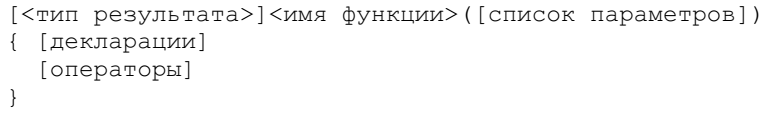
\includegraphics[scale=0.5]{images/lec03-pic01.png}
\end{figure}
Возврат значения функцией 
\begin{itemize}
\item return <выражение>;
\item по умолчанию - возвращаемое значение типа int;
\item void - отсутствие возвращаемого значения.
\end{itemize}
\end{frame}

\begin{frame}
Прототим - описание функции, средство контроля за соответствием фактических параметров в вызове функции ее формальным параметрам.
\begin{figure}[h]
\centering
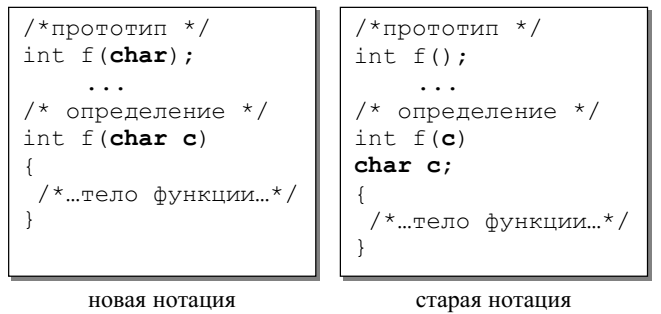
\includegraphics[scale=0.5]{images/lec03-pic02.png}
\end{figure}
Прототип 
\begin{itemize}
\item нужен, если вызов встречается до определения;
\item если прототип отсутствует? функция, которая возвращает int;
\item int foo() и int foo(void);
\item аргументы всегда передаются в функцию 'по значению';
\end{itemize}
\end{frame}

\begin{frame}
\textbf{Задача}. Написать функцию, суммирующую два вещественных значения в двух вариантах: сумма – возвращаемое значение функции и сумма – параметр функции.
\begin{figure}[h]
\centering
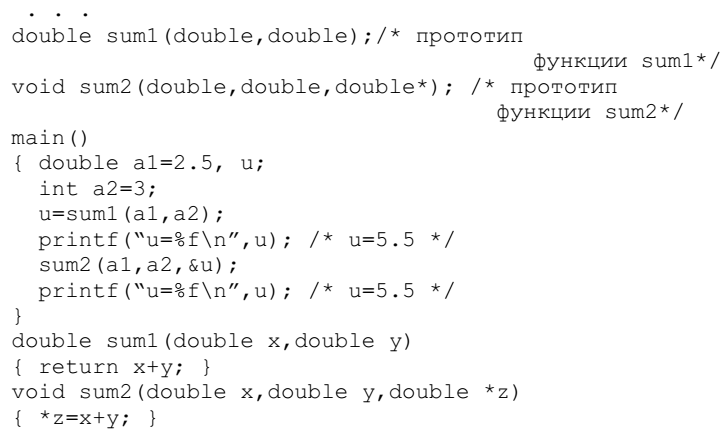
\includegraphics[scale=0.5]{images/lec03-pic03.png}
\end{figure}
\end{frame}

\begin{frame}
Список параметров переменной длины
\begin{figure}[h]
\centering

\includegraphics[scale=0.5]{images/lec03-pic04.png}
\end{figure}
Использование

\begin{itemize}
\item функции не известны ни типы передаваемых неименованных параметров, ни их количество;
\item подключить стандартную библиотеку stdargs.h;
\item описатьпеременную типа va\_list;
\item обратиться к макросу va\_start;
\item получать значение следующего параметра - va\_arg;
\item завершение - va\_end;
\end{itemize}

\begin{figure}[h]
\centering
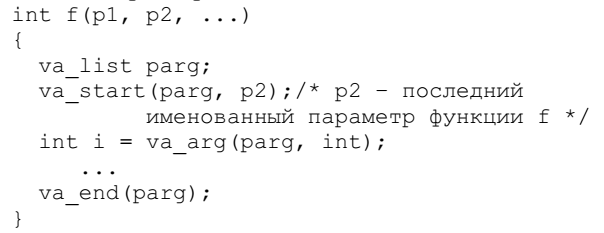
\includegraphics[scale=0.5]{images/lec03-pic05.png}
\end{figure}
\end{frame}

\begin{frame}
Общая структура программы
\begin{itemize}
\item может размещаться как в одном, так и в нескольких файлах;
\item может содержать одну или несколько функций;
\item одна из которых считается главной (main) - точка входа в программу;
\item определение каждой функции должно полностью размещаться в одном файле;
\item один этом файл может содержать несколько определений различных функций.
\end{itemize}
Характеристики переменных
\begin{itemize}
\item область видимости;
\item область существования.
\end{itemize}
\end{frame}

\begin{frame}
\begin{block}{Область видимости переменной}
определяет часть исходного текста программы, из любой точки которой доступна данная переменная.
\end{block}
\begin{itemize}
\item видимые в пределах блоков (локальные);
\item видимые в пределах файла;
\item видимые в пределах программы.
\end{itemize}
\end{frame}

\begin{frame}
Для переменных, определенных в начале любого блока, областью видимости является весь этот блок. 

В случае вложенных блоков переменные, определенные внутри вложенного блока, 'перекрывают' переменные с такими же именами, определенные в объемлющем блоке (и так для любой степени вложенности).
\begin{figure}[h]
\centering
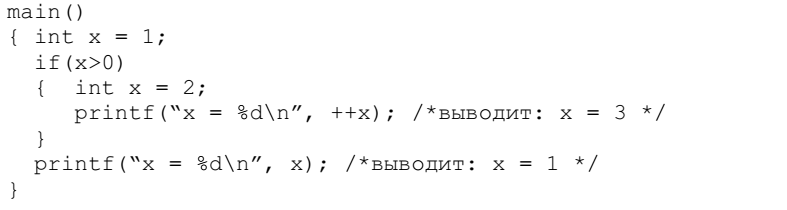
\includegraphics[scale=0.5]{images/lec03-pic06.png}
\end{figure}
\end{frame}

\begin{frame}
Переменные, определенные внутри функции, “перекрывают” формальные параметры с теми же именами.
\begin{figure}[h]
\centering
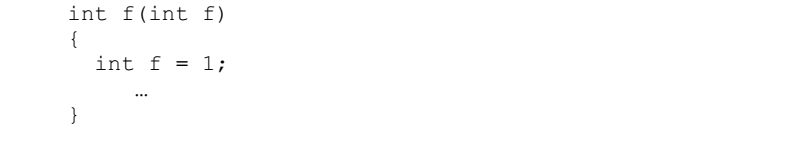
\includegraphics[scale=0.5]{images/lec03-pic07.png}
\end{figure}
\end{frame}

\begin{frame}
Переменные, определенные вне блоков (т.е., фактически, вне тела какой-либо функции), доступны с точки определения до конца файла. Если на такую переменную нужно сослаться до того, как она определена, необходимо ее описание со спецификатором extern.
\begin{figure}[h]
\centering
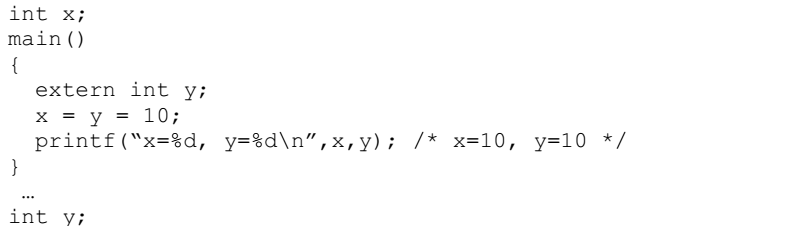
\includegraphics[scale=0.5]{images/lec03-pic08.png}
\end{figure}
\end{frame}

\begin{frame}
В файле вне функций не может встречаться несколько определений переменных (возможно, разных типов) с одним и тем же именем.
\begin{figure}[h]
\centering
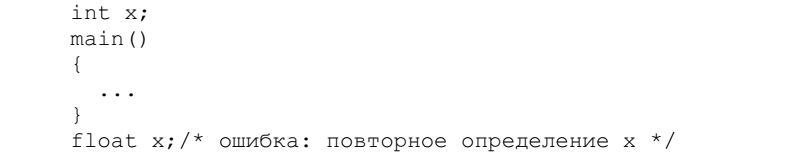
\includegraphics[scale=0.5]{images/lec03-pic09.png}
\end{figure}
Указание static, примененное к нелокальной переменной или функции, ограничивает область их видимости концом файла.

Если используемая переменная определена в другом программном файле, она также должна быть описана со спецификатором extern. При таком описании переменной память под нее не отводится, а только декларируется тип переменной, что позволяет
компилятору осуществлять проверки типизации.
\end{frame}

\begin{frame}
\begin{block}{Область существования переменной}
множество всех точек программы, при приходе управления на которые переменная
существует, т.е. для нее выделена память.
\end{block}
Статические переменные
\begin{itemize}
\item существуют на всем протяжении работы программы;
\item выделяется на этапе редактирования внешних связей и загрузки программы;
\item тогда же происходит и инициализация статических переменных;
\item инициализатором для статической переменной может служить только константное выражение;
\item при отсутствии инициализатора статические переменные по умолчанию инициализируются нулем;
\item все переменные, определенные вне функций, являются статическими.
\end{itemize}
\end{frame}

\begin{frame}
Определение статической переменной, локализованной в блоке
\begin{figure}[h]
\centering
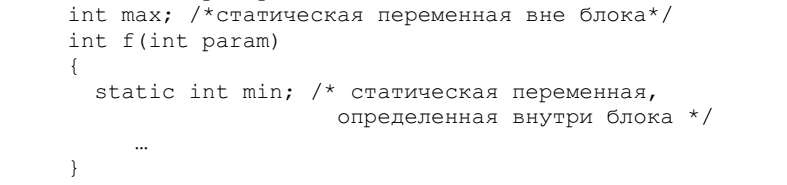
\includegraphics[scale=0.5]{images/lec03-pic10.png}
\end{figure}
\end{frame}

\begin{frame}
Сохранение значений статической переменной при выходе из блока
\begin{figure}[h]
\centering
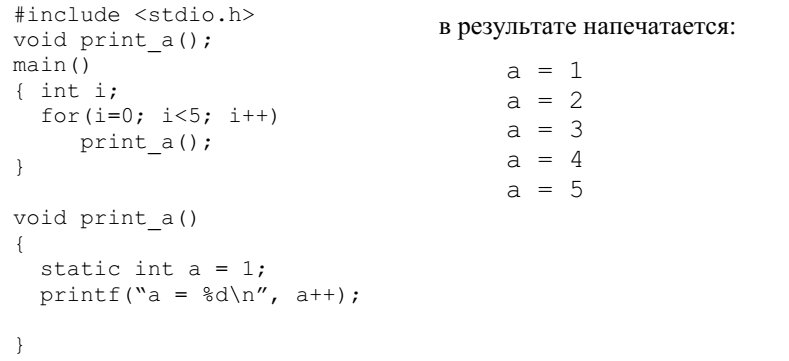
\includegraphics[scale=0.5]{images/lec03-pic11.png}
\end{figure}
\end{frame}

\begin{frame}
Автоматические переменные
\begin{itemize}
\item все переменные определенные внутри блока (функции) и не являющиеся статическими;
\item существуют на протяжении работы блока, в котором они определены, включая блоки, вложенные в данный. 
\item выделение памяти под автоматические переменные и их инициализация осуществляется каждый раз при входе в блок;
\item инициализация для автоматических переменных, фактически, эквивалентна
присваиванию, т.е. в качестве инициализирующего выражения может выступать любое выражение, которое может стоять в правой части оператора присваивания;
\item при отсутствии инициализатора начальное значение по умолчанию для автоматических переменных не определено.
\end{itemize}
\end{frame}

\begin{frame}
\begin{figure}[h]
\centering
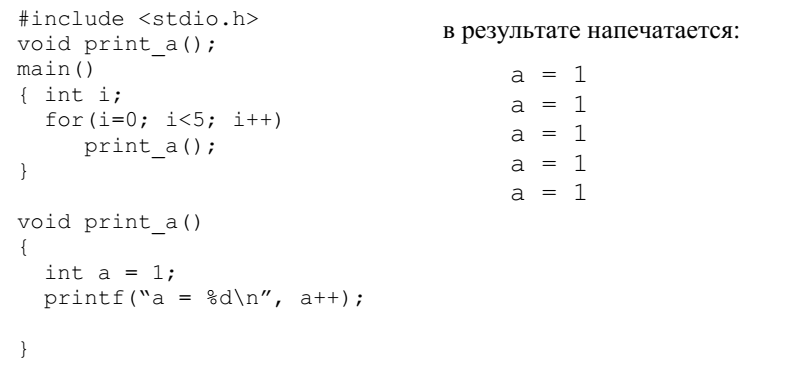
\includegraphics[scale=0.5]{images/lec03-pic12.png}
\end{figure}
\end{frame}

\begin{frame}
Регистровые переменные
\begin{itemize}
\item квалификатор register в определении переменных указывает компилятору, что данную переменную в целях ускорения программы имеет смысл разместить на регистрах, однако компилятор может проигнорировать это указание;
\item может применяться только к автоматическим переменным и формальным параметрам функций;
\item для регистровых переменных не определено понятие адреса  (т.е. не определена операция \&).
\end{itemize}
\end{frame}

\begin{frame}
\begin{figure}[h]
\centering
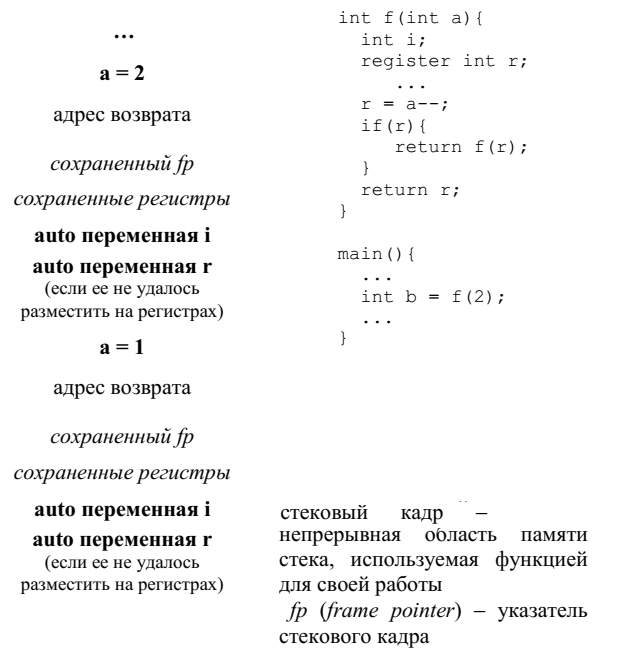
\includegraphics[scale=0.5]{images/lec03-pic13.png}
\end{figure}
\end{frame}

\section{Препроцессор}

%\section{Указатели и массивы}
%\section{Указатели на функцию. Сложные декларации}
%\section{Структуры и объединения}
%\section{Файлы} 

\end{document}
